\documentclass{article}


\usepackage{arxiv}

\usepackage[utf8]{inputenc} % allow utf-8 input
\usepackage[T1]{fontenc}    % use 8-bit T1 fonts
\usepackage{hyperref}       % hyperlinks
\usepackage{url}            % simple URL typesetting
\usepackage{booktabs}       % professional-quality tables
\usepackage{amsfonts}       % blackboard math symbols
\usepackage{nicefrac}       % compact symbols for 1/2, etc.
\usepackage{microtype}      % microtypography
\usepackage{lipsum}
\usepackage{graphicx}
\usepackage{epstopdf}
\usepackage{amsmath}
\usepackage{float}
\usepackage{svg}
\usepackage{capt-of}

\pdfminorversion=7

\graphicspath{{./graphics/}}
\epstopdfsetup{outdir=./}
\svgpath{./graphics/}

\title{\textbf{Nucleic Transformer: DNA sequence classification with self-attention on k-mer graphs}}


\author{
  Shujun He \\
  Department of Chemical Engineering\\
  Texas A\&M University\\
  College Station, TX\\
  \texttt{shujun@tamu.edu} \\
  %% examples of more authors
    \And
  Baizhen Gao \\
  Department of Chemical Engineering\\
  Texas A\&M University\\
  College Station, TX\\
  \texttt{baizhen@tamu.edu } \\ 

    \And
  Rushant Sabnis \\
  Department of Chemical Engineering\\
  Texas A\&M University\\
  College Station, TX\\
  \texttt{rushantsabnis@tamu.edu} \\   

   \And
  Qing Sun \\
  Department of Chemical Engineering\\
  Texas A\&M University\\
  College Station, TX\\
  \texttt{sunqing@tamu.edu} \\
  %% examples of more authors
  %% \AND
  %% Coauthor \\
  %% Affiliation \\
  %% Address \\
  %% \texttt{email} \\
  %% \And
  %% Coauthor \\
  %% Affiliation \\
  %% Address \\
  %% \texttt{email} \\
  %% \And
  %% Coauthor \\
  %% Affiliation \\
  %% Address \\
  %% \texttt{email} \\
}



\AtBeginDocument{\hypersetup{pdfborder={0 0 0}}}% <-----------
\begin{document}
\maketitle
\begin{abstract}

\end{abstract}


% keywords can be removed
\keywords{Deep learning \and Natural Language Processing \and Neural Network \and Bioinformatics}


\section{Introduction}

%Methods
\section{Methods}
Unlike other work in the literature involving promoter classification, our method requires minimal preprocessing and makes predictions directly from raw DNA sequences (Figure \ref{fig:network_architecture}). The key ideas that contribute to the effectiveness and novelty of our approach include:
\begin{itemize}
\itemsep0em 
\item Using 1-D convolutional layers to aggregate DNA k-mers 
\item Using state of the art NLP architecture: transformers, 
\item Artificial injection noise into the training process for more robust learning
\end{itemize}

\begin{figure}[H]
\center
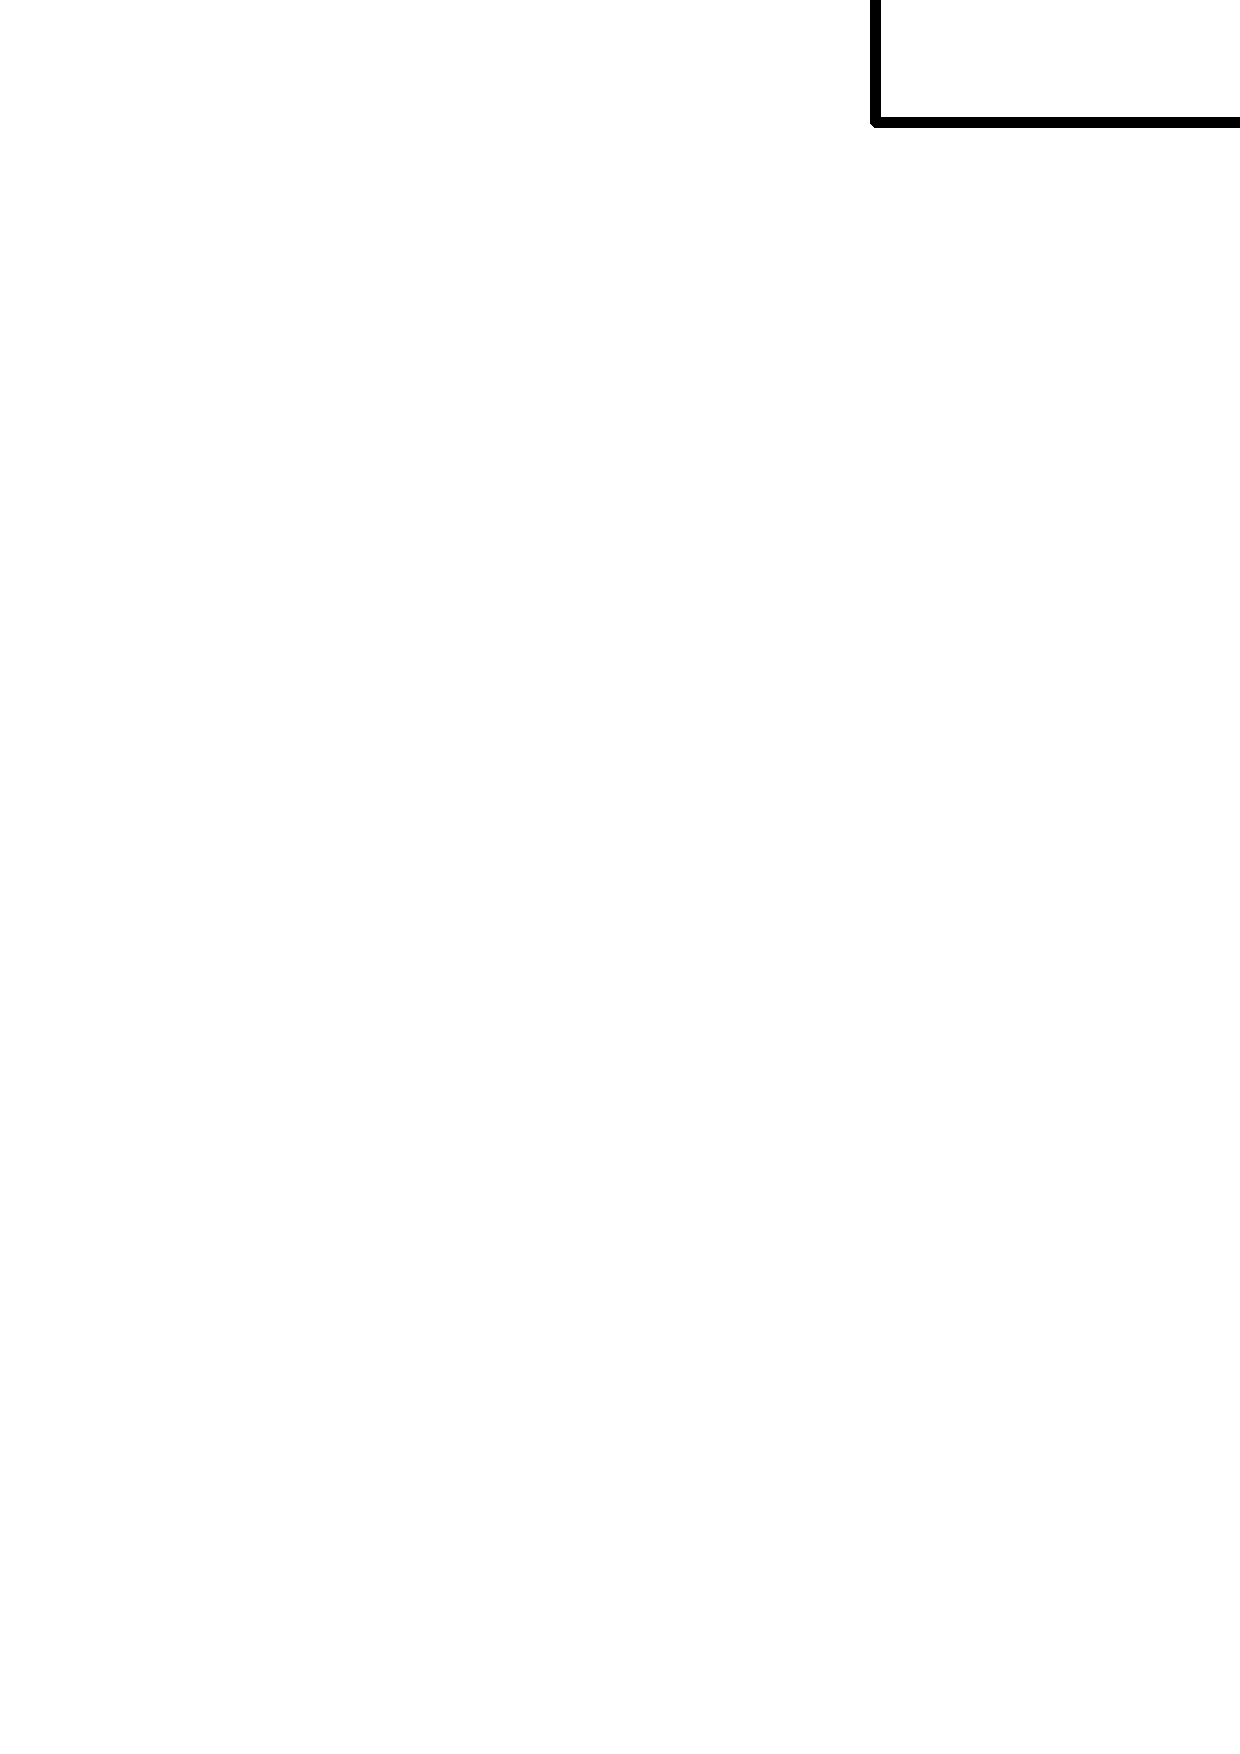
\includegraphics[width=0.9\textwidth]{network_architecture}
\caption{\textbf{Placeholder} Summary of methods}
\label{fig:network_architecture}
\end{figure}

%Benchmark dataset
\subsection{Benchmark dataset}
High quality and accessible datasets are imperative in advancing bioinformatics, not only because of the useful information they provide but also because they establish benchmarks where fair comparisons between different models can be made. In this work, we use 3 high quality and easily accessible datasets that have been studied in the literature, which include a labeled \textit{E.Coli} promoter/non-promoter dataset, a labeled viral/non-viral genome dataset, and a dataset with species labels. 

%promoter/non-promoter dataset
\subsubsection{\textit{E.Coli} promoter/non-promoter dataset}
The \textit{E.Coli} promoter/non-promoter dataset used is an experimentally confirmed benchmark dataset widely used in the literature to model and evaluate DNA promoter sequences \cite{ipsw}. All DNA sequences in the dataset are collected from RegulonDB, and sequences are screened by CD-HIT based on redundant sequence identity \cite{cdhit}. This dataset consists of 3,382 promoter sequences and 3,382 non-promoter sequences. The 3,382 promoter sequences can be further divided into 1,591 strong promoters and 1,792 weak promoters. This dataset can be freely downloaded at \href{http://www.jci-bioinfo.cn/iPSW(2L)-PseKNC/images/Supp.pdf}{http://www.jci-bioinfo.cn/iPSW(2L)-PseKNC/images/Supp.pdf}. Model performance is evaluated using 5-fold cross validation, where the data is split using iterativte stratification \cite{iter_strat}.


\subsubsection{Viral/non-viral genome dataset}


\subsubsection{Dataset with species labels}




%DNA as a language
\subsection{DNA as a language}
Any DNA seqeuence is a sequence of nucleotides, each of which can be one of A (adenosine), C (cytidine), G (guanosine), and T (thymine). Therefore, if we consider DNA a langauge that uses only four different words to encode information, we can model it in similar fashion as a natural langauge. This idea then allows us to agnostically apply Natural Language Processing (NLP) techniques in the domain of deep learning without injection of domain specific knowledge in bioinformatics.  

Although there are similarities between DNA sequences and natural language, there are also some important differences. Take the English language for example, all words in the vocabulary are combinations of the 26 letters in the alphabet; similarly, a DNA sequence is a sequence of 4 nucleotides. Nevertheless, the English langauge not only contains letters but also spaces that separate words, and commas and periods that seperate sentences, whereas comparatively a DNA sequence consists of only 4 letters. Further, when humans interpret a sentence, words are discretely recognized and each word can be considered a discrete object. As a result, state of art NLP models evaluate languages as collections of words (and punctuations) instead of letters. Since a DNA sequence does not have punctuations, we need to find a way to transform a DNA sequence into "words", which we will discuss in detail in the next section.


%K-mer with 1-D convolutional layers
\subsection{K-mers with 1-D convolutions}
A common method to process DNA sequences in the field of bioinformatics is to transform them into k-mers. For instance, consider a short DNA sequence ATGC. The k-mers in this sequence are subsequences of length k, so ATGC has three 2-mers AT, TG, and GC, two 3-mers are ATG and TGC, and one 4-mer ATGC. Converting a DNA sequence into k-mers is analogous to separating a language sentence into words and allows for more efficient extraction of information from DNA.

The extraction of k-mers from a DNA sequence can be considered a sliding window of size $k$ taking snapshots of the sequence while moving one space at a time from one end of the sequence to the other, which is conceptually identical to the convolution operation used in deep learning. Consider a simple example of convolution involving a vector $S\in \mathcal{R}^l$, where $l$ is the length of the vector, and a convolution kernel $K\in \mathcal{R}^3$, which convolves over the vector $S$. If the convolutional kernel strides one position at a time, an output vector of dot products $O\in \mathcal{R}^{l-2}$ is computed,
\begin{equation}
O_p= \sum_{i \in \{0,1,2\}} K_i S_{p+i},
\end{equation}
where $p$ denotes the position in the output vector. In this case, the convolution operation aggregates local information with 3 positions at a time, so if $S$ is a sequence of nucleotides, the convolution operation is essentially extracting 3-mers from the DNA sequence $S$. Consequently, it is conceptually clear that a convolution kernel of size k can be used to transform a DNA sequence into k-mers. In the next paragraph, we will explain further how this works mathematically. 

Since our model takes sequences of DNA nucleotides as input, we first transform each nucleotide into embeddings of fixed size $d_{model}$. So now for each sequence we have a tensor $I \in  \mathcal{R}^{l\times d_{model}}$, where $l$ is the length of the sequence. Because we are using the transformers as the encoder, which is permutation invariant, we need to add positional encoding, same as the implementation in \cite{transformer_paper}:

\begin{align}
PE_{(pos,2i)}=sin(pos/5000^{2i/d_{model}})\\
PE_{(pos,2i+1)}=sin(cos/5000^{2i/d_{model}}),
\end{align}

where $pos$ is the position and $i$ is the channel dimension. Now to aggregate k-mers we perform convolutions of different kernel sizes on the tensor $I$ without padding and stride = 1. For each time convolution operation with kernel size $k$ is performed over $I$, a new tensor $K_k \in \mathcal{R}^{(l-k+1)\times d_{model}}$ representing the sequence of k-mers is generated. Now we simply concatenate all k-mer tensors $\{K_0...K_{k_{max}}\}$, where $k_{max}$ denotes the tensor representing the sequence of largest k-mers, in the first dimension to aggregate k-mers sequences. Finally, we obtain a collection of k-mers, where each k-mer is represented by a feature vector of size $d_{model}$.


%K-mer with 1-D convolutional layers
\subsection{K-mers with 1-D convolutions compared to k-mer embeddings}
Indeed our representation of k-mers deviates from conventional representation of words in deep learning, where each word in the vocabulary directly corresponds to a feature vector in a look up table. The disadvantage of using look up tables for k-mers is that a very small percentage of all possible k-mers are present in any dataset, and there is no way for the network to generalize to unseen k-mers. For instance, if a common promoter motif TATAAT appears in the dataset but a similar motif TATATT does not, there is no way for the network to generalize to the unseen motif TATATT, but using convolutions, it is easy for the network to recognize that there is not much difference between TATAAT and TATATT, leading to better generalization. Additionally,  embeddings of k-mers of larger sizes require a prohibitively large amount of parameters, since the total possible amount of k-mers for is $4^k$. Therefore, we can calculate the number of parameters needed to represent k-mers with convolutions (assuming we use single nucleotide embeddings before convolution) and embeddings:

\begin{align}
N_{embedding}=d_{model}\times4^k \\
N_{convolution}=d_{model}^2\times k
\end{align} 

In most of our experiments, $d_{model}$ is set to 512, so we can plot and compare the number of parameters required k-mer representations using embeddings and convolutions (Figure \ref{fig:kmer parameters}), where $N_{embedding}$ scales exponentially with $k$. 


\begin{figure}[H]
\center
%\vspace{0pt}
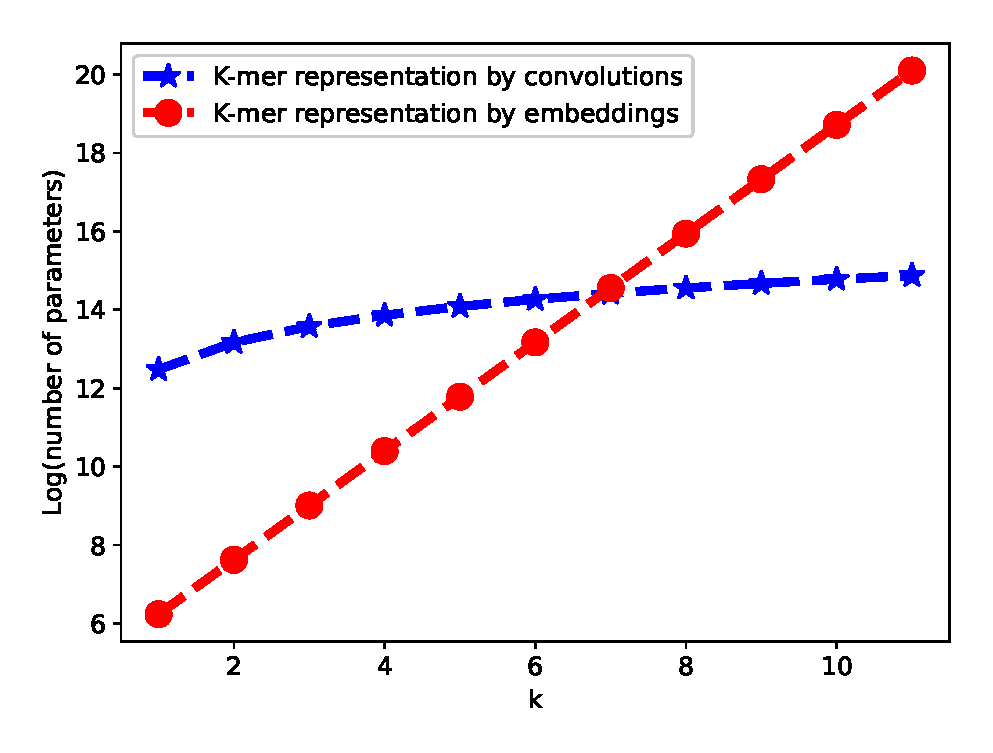
\includegraphics[width=0.8\textwidth]{kmer_parameter_complexity.eps}
%\includesvg{k_mer_aggregation}
\caption{Scaling of number of parameters required to represent k-mers with embeddings vs convolutions. Calculations are done with $d_{model}=512$.}
\label{fig:kmer parameters}
\end{figure}
 



%Core architecture: transformers
\subsection{Transformers and multi-head self-attention}
For the encoder, we implement the vanilla transformer encoder \cite{transformer_paper}, which uses the multi-head self-attention mechanism. Unlike a single-head attention function, the multi-head self-attention function linearly projects $d_{model}$-dimensional keys, values and queries into lower dimensional representations. Then the multi-head attention function directly operates on the entire sequence. It has been posited that the multi-head mechanism allows different heads to learn different hidden representations of the input, leading to better performance. The multi-head self-attention mechanism can be summarized in a few equations:
\begin{align}
\text{Attention}(Q,K,V)=\text{softmax}(\frac{QK^T}{\sqrt{d_k}})V \\
\text{MultiHead}(Q,K,V)=\text{Concat}(head_1,...,head_h)W^O \\
\text{where $head_i$}=\text{Attention}(QW^Q_i,KW^K_i,VW^V_i).
\end{align}
Our implementation of the transformer encoder is exactly the same as the original transformer paper. Since we are only using the transformer encoder, $Q,K,V$ come from the same sequence of feature vectors (hence the name self-attention), each of which represents a k-mer with positional encoding. 

The self-attention mechanism enables each k-mer to attend to all k-mers (including itself), so global dependencies can be drawn between k-mers of any size at any distance (Figure \ref{fig:global}). Contrary to recurrence and convolutions, both of which enforce sparse local connectivity, transformers allow for dense or complete global connectivity. The ability to draw global dependencies of transformers is a huge advantage over recurrence and convolutions, both of which struggle with long sequences. 


\begin{figure}[H]
\center
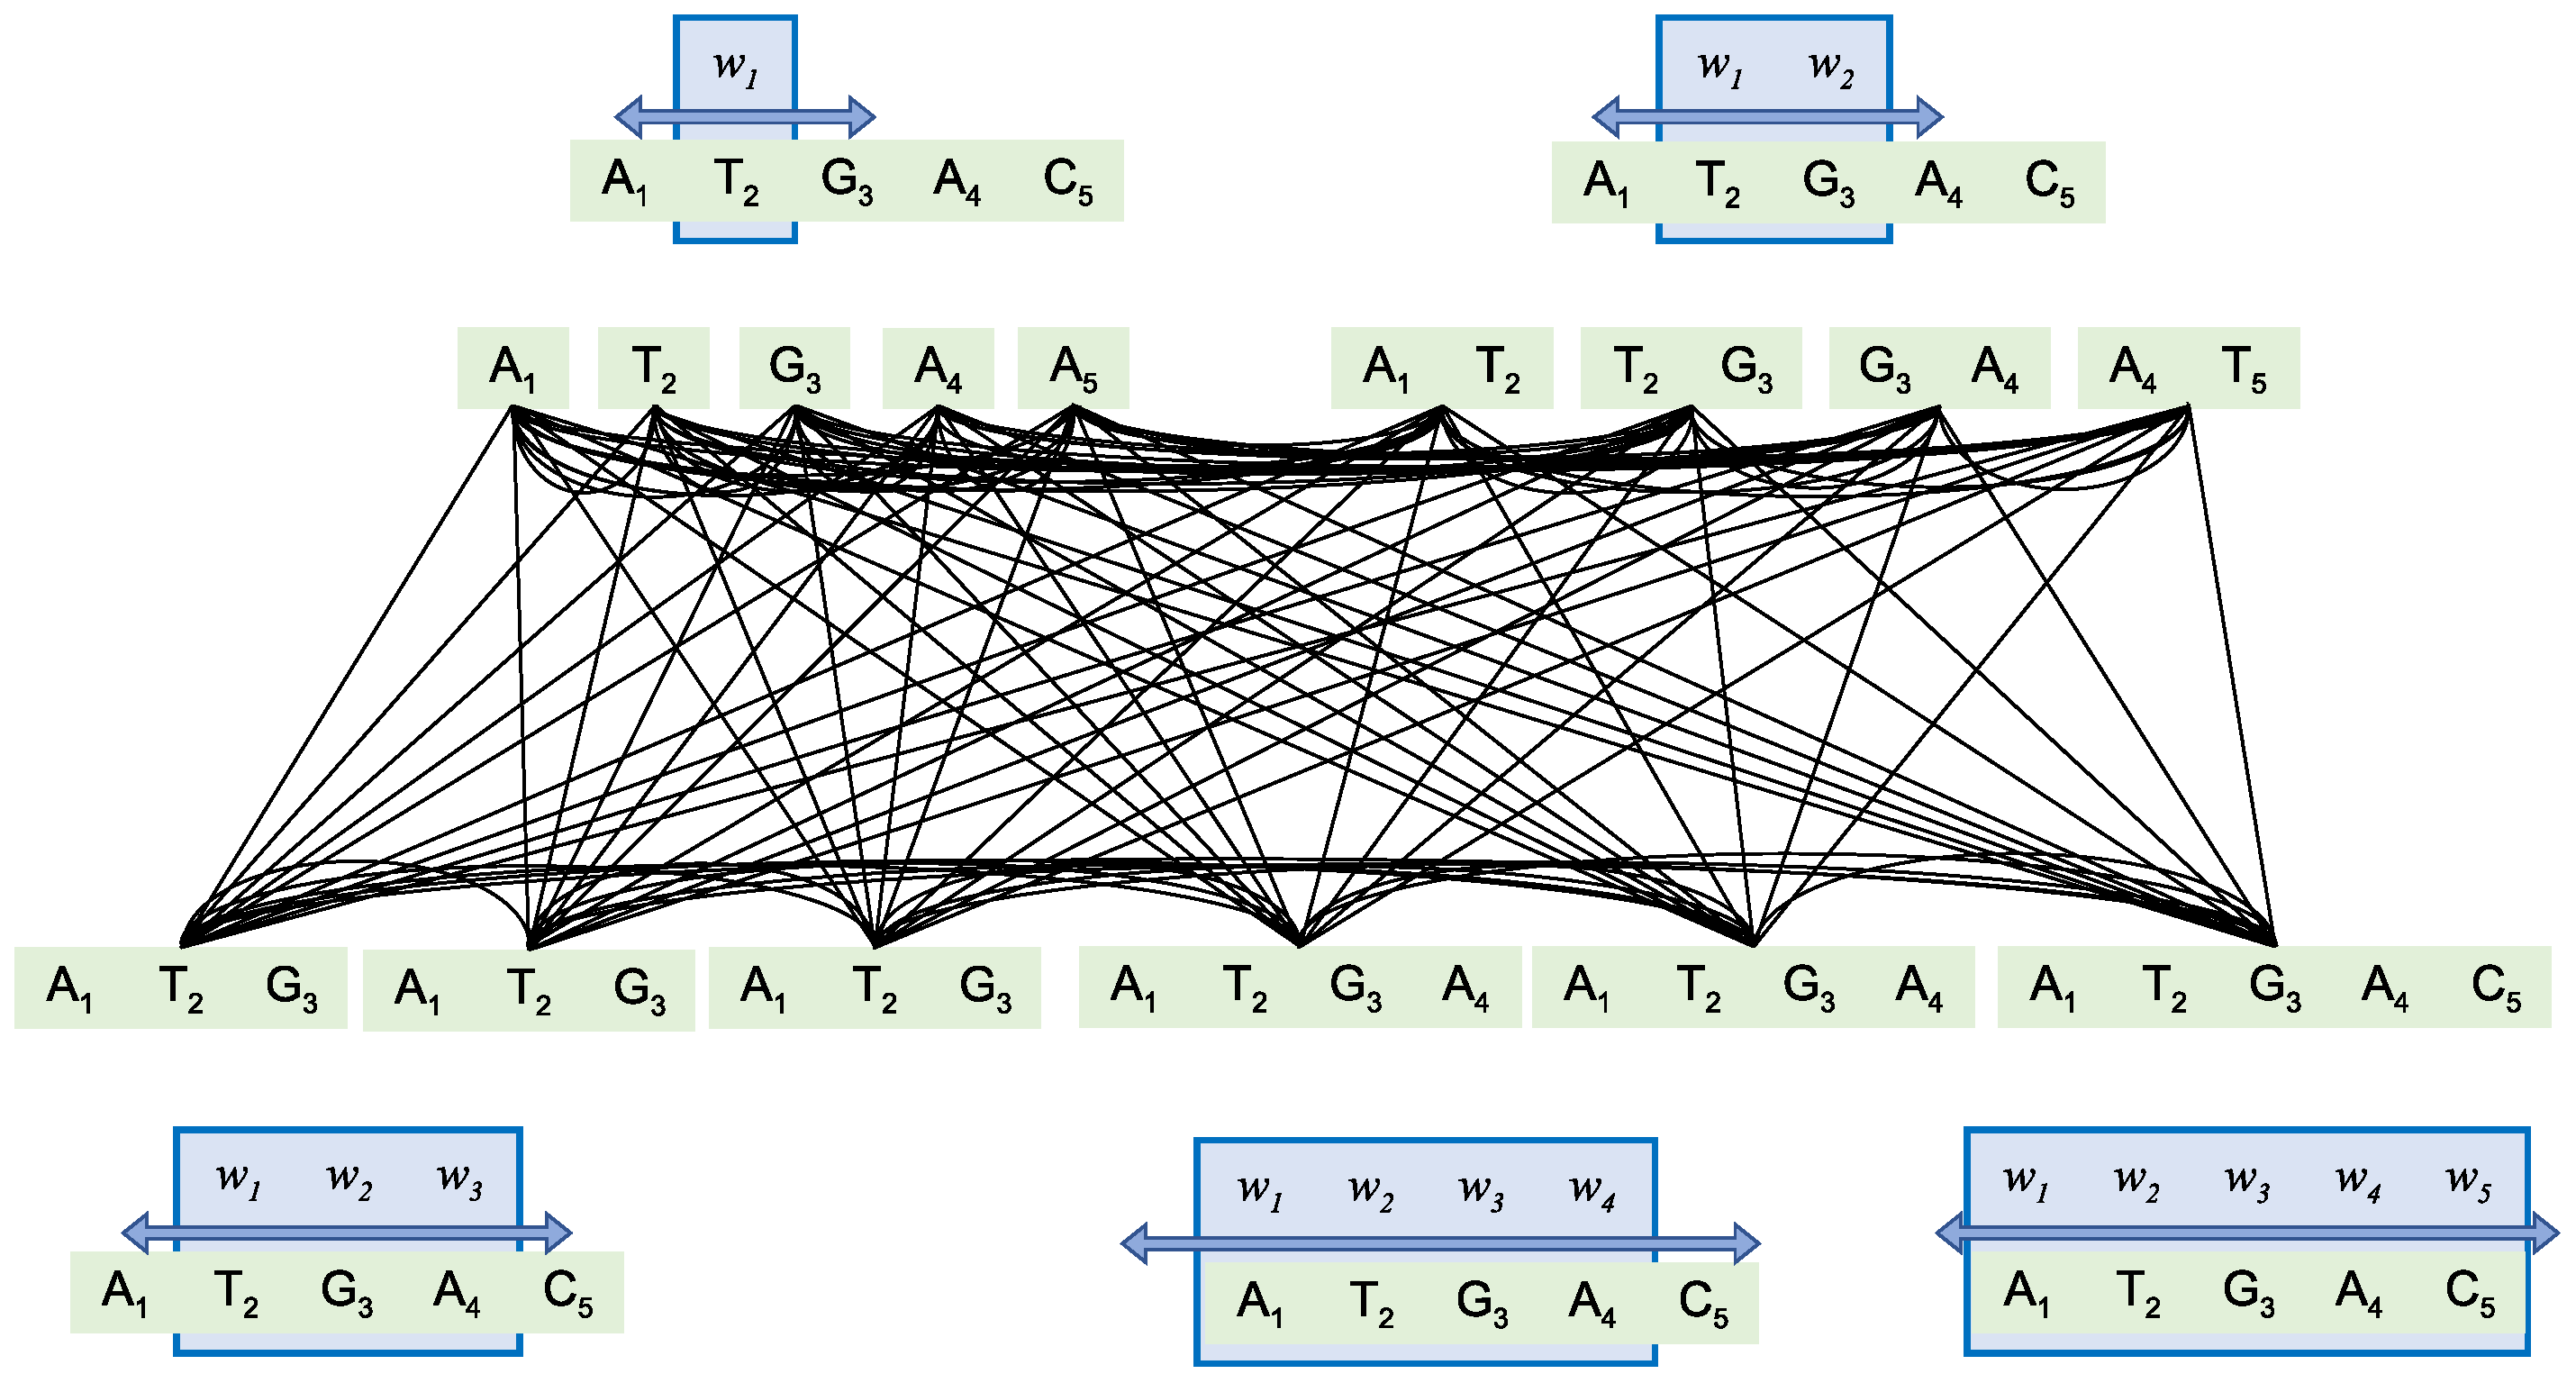
\includegraphics[width=1\textwidth]{k_mer_aggregation.eps}
%\includesvg{k_mer_aggregation}
\caption{\textbf{Placeholder} K-mers are extracted from the source sequence "ATGAC" and aggregated. The transformer then allows each k-mer to attend to all k-mers in the source sequence.}
\label{fig:global}
\end{figure}


%K-mer graphs/meta-graphs
\subsection{Computational complexity of k-mer graphs and meta-graphs}
In this work, we explore two different ways to construct the k-mer graphs as input into the transformer encoder, which we denote k-mer graphs and k-mer meta-graphs. K-mer graphs simply denote graphs of k-mers of the same size $k$ resulting from using 1-D convolutions with stride 1 on an input DNA sequence, whereas k-mer meta-graphs are graphs of k-mers of 1 through $k$ aggregated together. It is obvious that using k-mer meta-graphs is much more computationally expensive. For instance, comparatively a 2-mer graph has only approximately half of the vertices in a k-mer meta-graph of 2-mers and 3-mers. Since the transformer's self-attention function's computational complexity scales quadratically with the amount of vertices in the graph, the computational complexity of using k-mer meta-graphs is prohibitively high for larger datasets with longer sequences. Using the promoter dataset sequences as an example which are DNA sequences of length 81, if we consider computing one element in the self-attention weight matrix to have computational complexity of one, we can calculate the computational complexity of k-mer graphs and k-mer meta-graphs (Figure \ref{fig:graph complexity}). Using k-mer meta-graphs with larger $k$'s is very computationally expensive. Surprisingly, due to rapid development of GPU computing in recent years and the emergence of mixed precision computing enabled by Nvidia's tensor core technology, it is actually viable to train models from scratch using k-mer meta-graphs on small datasets. As a result, we only experimented with the k-mer meta-graphs on the \textit{E.Coli} promoter/non-promoter dataset, which is smallest dataset we used in this study. For the other two datasets used in this study, all experiments were conducted with k-mer graphs as input to the transformer encoder. 

\begin{figure}[H]
\center
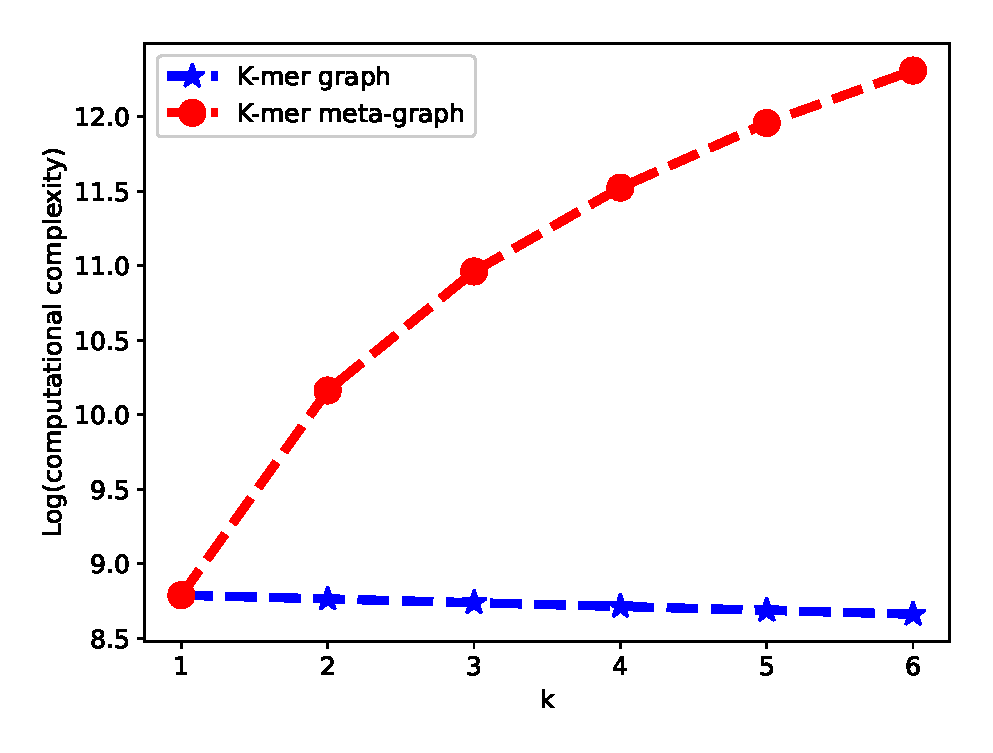
\includegraphics[width=0.8\textwidth]{graph_metagraph_complexity.eps}
%\includesvg{k_mer_aggregation}
\caption{Computational complexity of k-mer graphs vs k-mer metagraphs. Computing one element of the attention weight matrix is considered to have a computational complexity of one, and computational complexity calculations are done accordingly. }
\label{fig:graph complexity}
\end{figure}


%K-mer aggregation and self-attention allow interpretability
\subsection{K-mer meta-graph and interpretability}
Our representation of a DNA sequence can be considered a k-mer meta-graph, where vertices can be sets of vertices. If we consider the single nucleotides the fundamental vertices of the metagraph, the k-mers where $k > 1$ are meta-vertices. Each vertex (including meta-vertices) are represented as a feature vector within the transformer. Since we do not use attention masks, our graphs are complete graphs with self connection.  Therefore, for a graph with $N$ vertices, the transformer attention function generates an attention weight matrix of dimensions $N\times N$, where the second dimension is normalized by a softmax function. Depending on how many k-mers of different lengths are aggregated, the size of the meta-graph $N$ can be several times larger than the original sequence $L$. 

By visualizing the attention weight matrix as a square image with $N\times N$ pixels, we can directly see which k-mers the transformer considers important by the magnitude of attention weights corresponding to k-mers. Since softmax function is used on the second dimension of the weight matrix, each row of the attention weight matrix sums up to 1; however, if we sum the attention weight matrix by the first dimension, we can evaluate how much attention in total each k-mer receives in a given attention function. 

Considering the size of meta-graphs, visualizing the complete $N\times N$ attention weight matrix is unreasonable for meta-graph interpretability. So we introduce a way to reduce the meta-graph $N\times N$ attention weight matrix back to an $L\times L$ matrix, where each element represents the attention weight between a pair of single nucleotides. Any single element in the $N\times N$ attention weight matrix of the meta-graph corresponds to a pair of vertices representing two k-mers, $V_{k_1}^{pos_1}$ and $V_{k_2}^{pos_2}$, where $k_i$ denotes the size of k-mer vertex, and $pos_j$ denotes the starting position (first single nucleotide) of the k-mer. Since each k-mer vertex is an aggregation of locally connected single nucleotides, $V_{k_i}^{pos_j}$ corresponds to a section of the source DNA sequence starting from position $j$ and ending at position $j+i$. Then a pair of vertices (e.g. $V_{k_1}^{pos_1}$ and $V_{k_2}^{pos_2}$) corresponds to a rectangular region of the $L\times L$ attention weight matrix. In the case of $k_1 > 1 \ \& \ k_2 = 1$ or $k_1 = 1 \ \& \ k_2 > 1$, the pair of vertices corresponds to a slice (or vector) in the $L\times L$ attention weight matrix. If both $k_1$ and $k_2$ are 1, the pair of vertices correspond to a single element in the $L\times L$ attention weight matrix. In summary, to transform the meta-graph attention weights matrix back to an $L\times L$ matrix:
\begin{enumerate}
\item Initialize a matrix of dimensions $L\times L$ with all elements set to 0
\item Add each element in the $N\times N$ attention weight matrix back to the corresponding region in the $L\times L$ attention weight matrix
\end{enumerate}


%Artificial noise injection
\subsection{Artificial injection of noise}
There is no question that the transformer architecture is extremely powerful. In fact, it has been shown that the transformers can learn from the English Wikipedia which contains billions of words in an unsupervised fashion and achieve state-of-the-art results by finetuning on task specific data \cite{bert_paper}. It is known that deep learning models can perfectly memorize completely random data and labels, so to combat the memorization effect, we inject noise artificially by randomly mutating positions in the source DNA sequence before forward and backward propagation during training, similar to \cite{bert_paper}. It is true that these random mutations could be non-label-preserving; however, deep learning algorithm is known to be robust to massive label noise, so the non-label-preserving mutations should simply be ignored by the network during training \cite{RolnickVBS17}. The number of positions to randomly mutate is a hyperparamter that we denote $n_{mute}$, with which we experiment to find the best value. Note that in all our experiments, we simply randomly inject one of four nucleotides in randomly selected positions, and because we do not ensure nucleotide at each selected position is changed, the average amount of mutations is 3/4 of $n_{mute}$. 

%Multitasking learning
\subsection{Multitasking learning}
Because we are randomly mutating $n_{mute}$ random positions in the source sequence and the transformer encoder is effectively a sequence to sequence  architecture, we are able to add additional tasks aside from the main classification task. Specifically, we add two linear decoders, in addition to the linear decoder that classifies DNA sequences into promoter/non-promoter and strong/weak promoter. The first added decoder is trained to predict erroneous positions, and the second is trained to predict the correct nucleotides in erroneous positions. 


%Training details
\subsection{Training details}
Training of transformers can be tricky and wrong selection of training schedule and hyperparamters can be lead to diverged training \cite{trainingtipstransformers}, so here we detail the training process.

For the optimizer, we choose Adam \cite{adampaper}, a commonly used optimizer in deep learning with $\beta_1=0.9$, $\beta_2=0.99$, and $\epsilon=1e-8$. Weight decay is set to 0. Our learning rate schedule is a stepwise inverse square root decay schedule with warm up. Since we use a very small batch size of 24 during training, we adjust the learning rate by a scaling factor $C$:

\begin{align}
\text{learning rate}= C\cdot d_{model}^{-0.5}\cdot \text{min}(\text{step\_num}^{-0.5},\text{step\_num}\cdot \text{warmup\_steps}^{-1.5}).
\end{align}

In our experiments, $C$ is set 0.1 and warmup\_steps is set to 3200. Additionally, we use dropout \cite{dropoutpaper} of probability 0.1 in all attention layers, fully connected layers, positional encoding, and k-mer aggregation convolution layers.


%Results \& discussion
\section{Results \& discussion}
In this work, we experiment with a few different hyperparameters and then compare results using our best settings to other work in the literature. Subsequently, we visualize, analyze and interpret attention weight matrices.



\subsection{Promoter/non-promoter classification}
\subsubsection{Number of k-mers of different lengths aggregated}
To experiment with aggregating k-mers of different lengths, first we set a baseline with no k-mer aggregation, where only single nucleotides with positional encoding are inputted into the transformer. Then we incrementally add more k-mers vertices to the metagraph, where we add one set of larger k-mer vertices at a time, and evaluate the model performance (Figure \ref{fig:kmers}). Additionally, we also run experiments without the transformer encoder to see the improvement the transformer encoder gives, in which case the k-mer aggregation layer is simply followed a maxpooling and fully connected layer. Here we use $n_{mute}=18$, and six transformer encoder layers.

The model's performance improves initially upon adding more longer k-mers, and then saturates to a point where adding more longer k-mers no longer increases performance. We see that aggregating 1-8 mers actually led to a decrease in performance, likely due to overfitting resulting from large convolution kernels. Further, we see that the transformer encoder consistently gives a significant boost in accuracy. It is important to note that the more k-mers are aggregated, the more the network has to process, leading to increased computational complexity.  Therefore, in subsequent experiments, we only aggregate 1-6 mers, because adding 7-mers only provides a minimal increase in accuracy (+0.1\%) and higher computational complexity.
\begin{figure}[H]
\center
\includegraphics[width=0.8\textwidth]{kmer_test.eps}
%\includesvg{k_mer_aggregation}
\caption{Bar chart of accuracy vs the amount of k-mers aggregated. Baseline corresponds to model performance without k-mer aggregation, and 1-2mer corresponds to 1-mer,2-mer aggregated, 1-3mer corresponds to 1-mer, and 2-mer, and 3-mer aggregated, etc.}
\label{fig:kmers}
\end{figure}



\subsubsection{Number of random mutations during training}

Much like most tunable hyperparameters in deep learning, we see from our experiments that there is an optimal value for the number of random mutations during training (Figure \ref{fig:nmute}). Our experiments show that the model tends to significantly overfit to the training data when no random mutations are added during training. The model quickly converges to 1.0 accuracy and close to 0 loss, indicating that the model has simply memorized the training data. In addition, it is clear that too many mutations will lead to underfitting, as there is too much random noise during training leading to poor convergence. 

%nmute and nlayer plot
\begin{minipage}{.5\linewidth}
\begin{figure}[H]
\center
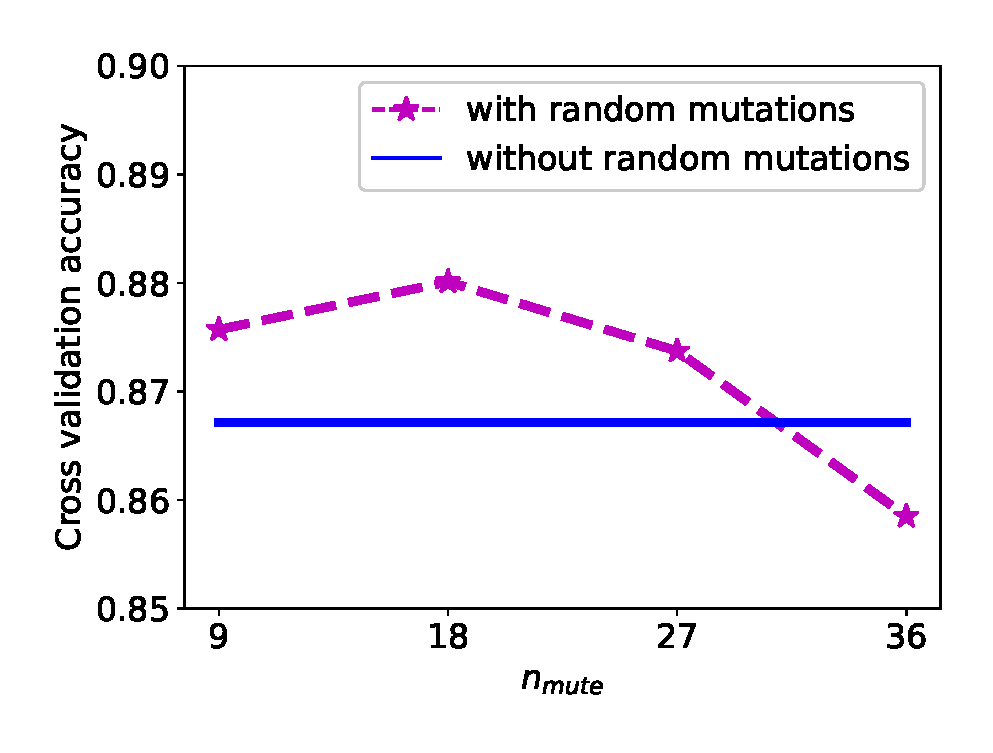
\includegraphics[width=1\textwidth]{nmute_test.eps}
%\includesvg{k_mer_aggregation}
\caption{Cross validation accuracy vs number of random mutations during training.}
\label{fig:nmute}
\end{figure}
  \end{minipage}%
\hspace{0.5cm}
  \begin{minipage}{.5\linewidth}
\begin{figure}[H]
\center
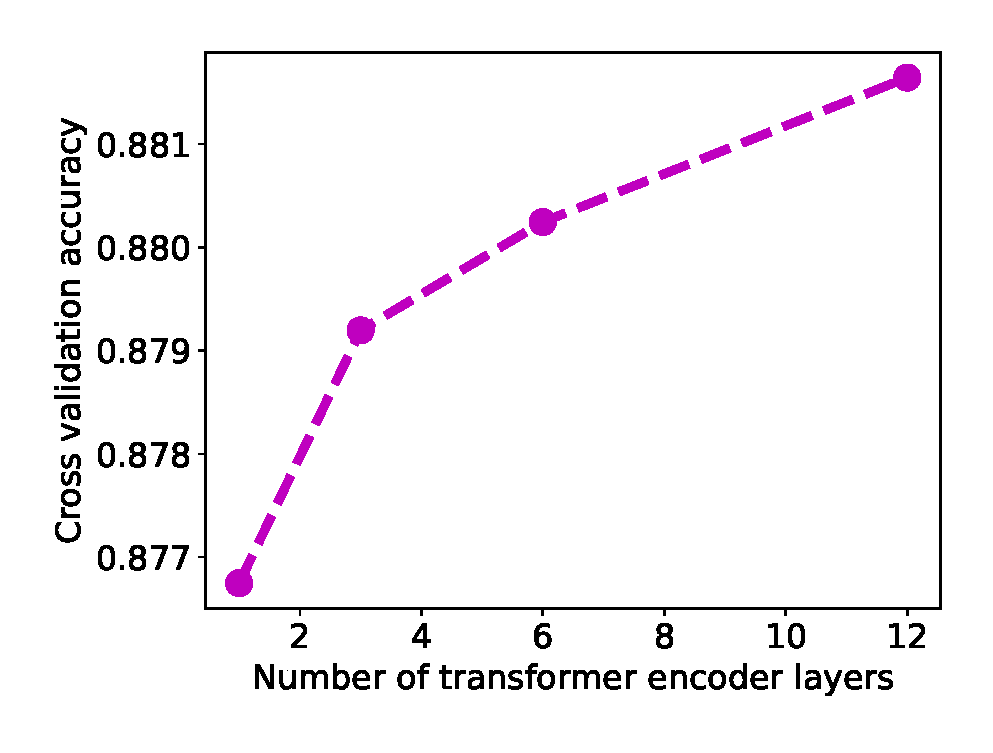
\includegraphics[width=1\textwidth]{layers_acc.eps}
%\includesvg{k_mer_aggregation}
\caption{Cross validation accuracy vs number of transformer encoder layers.}
\label{fig:nlayer}
\end{figure}
  \end{minipage}


\subsubsection{Number of transformer encoder layers}
Ever since the advent of residual connection introduced in Resnets\cite{resnetpaper1}, it has been known that in deeper learning systems, a deeper architecture always performs better than a shallower one, at least on the training set. On any sizable scale problems, increasing the capacity of the network architecture almost always leads to better performance as well. For example, OpenAI has recently trained a self-supervised transformer model GPT-2 \cite{GPT2}, which has 1.5 billion parameters. In this work, we also explore how a deeper transformer encoder compares to shallower ones. We see that even for a small scale problem of 5720 sequences, increasing the depth of the network still leads to improvement in accuracy (Figure \ref{fig:nlayer}). However, as the architecture gets deeper, there is diminishing returns, where the 12-layer transformer encoder only leads to a 0.1 \% improvement over the 6-layer transformer. 



\subsubsection{Comparison with top results in the literature}
\begin{table}[h]
\center
\begin{tabular}{@{}ccccc@{}}
\toprule
                    & Accuracy        & MCC             & Sensitivity     & Specificity     \\ \midrule
Nucleic Transformer & \textbf{0.8806} & \textbf{0.7612} & \textbf{0.8818} & \textbf{0.8794} \\
MULTiPly            & 0.8668          & 0.7224          & 0.8656          & 0.8668          \\
iPromoter-2L2.0     & 0.8498          & 0.6998          & 0.8413          & 0.8584          \\
iPromoter-2L1.0     & 0.8168          & 0.6343          & 0.792           & 0.8416          \\ \bottomrule
\end{tabular}
\caption{Performance of Nucleic Transformer against top results in the literature based on accuracy, MCC, sensitivity, and specificity.}
\label{tab:comparison}
\end{table}

\subsubsection{Independent test set results}


\subsubsection{Analysis of attention weights}



\subsubsection{Model behavior on randomly generated DNA sequences}
It has been experimentally shown that approximately 10\% random sequences can function as promoters \cite{denovo_promoters}. Here we screened one million randomly generated DNA sequences of length 81, and classified them with our trained model (Figure \ref{fig:random}). We found that despite a balanced distribution of positive and negative examples in the promoter/non-promoter dataset, our model recognized approximately 70\% of random DNA sequences as non-promoters. This suggests that our model is likely able to generalize well.  


\begin{figure}[H]
\center
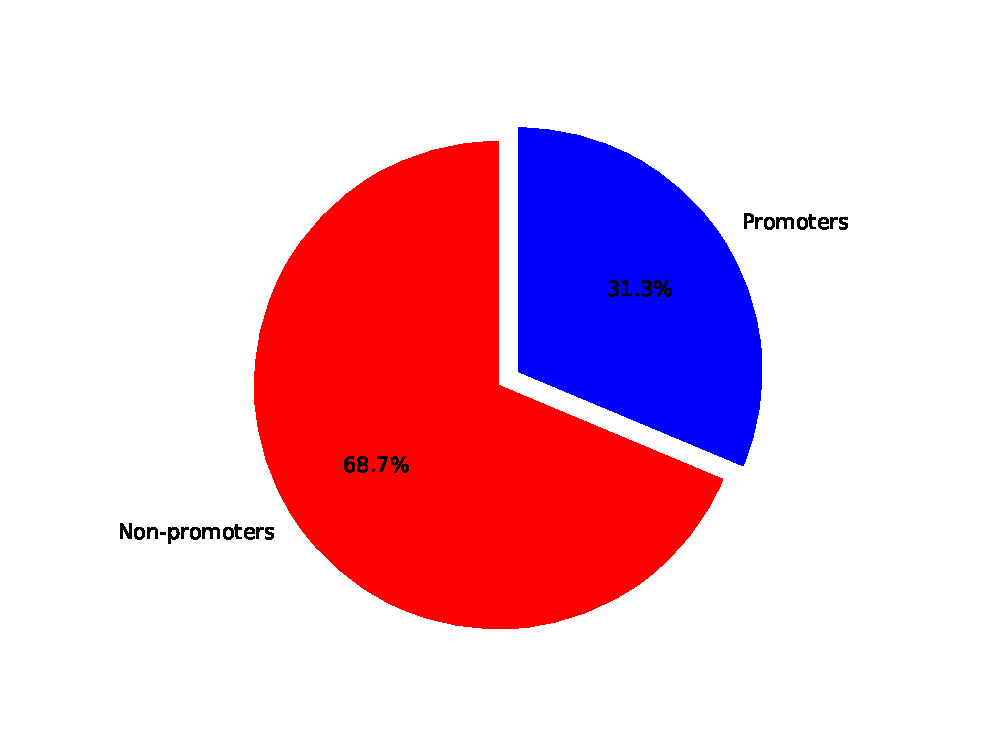
\includegraphics[width=0.8\textwidth]{massive_screening.eps}
%\includesvg{k_mer_aggregation}
\caption{}
\label{fig:random}
\end{figure}


%Viral/non-viral genome dataset
\subsection{Viral/non-viral classification}


\subsubsection{Comparison with Viraminer}
\begin{figure}[H]
\center
\includegraphics[width=0.8\textwidth]{viral_results.eps}
%\includesvg{k_mer_aggregation}
\caption{}
\label{fig:vs viraminer}
\end{figure}


\subsubsection{Effects of number of encoder layers}

\begin{figure}[H]
\center
\includegraphics[width=0.8\textwidth]{vira_layers.eps}
%\includesvg{k_mer_aggregation}
\caption{}
\label{fig:vira nlayer test}
\end{figure}


\subsubsection{Effects of size of $d_{model}$}

\begin{figure}[H]
\center
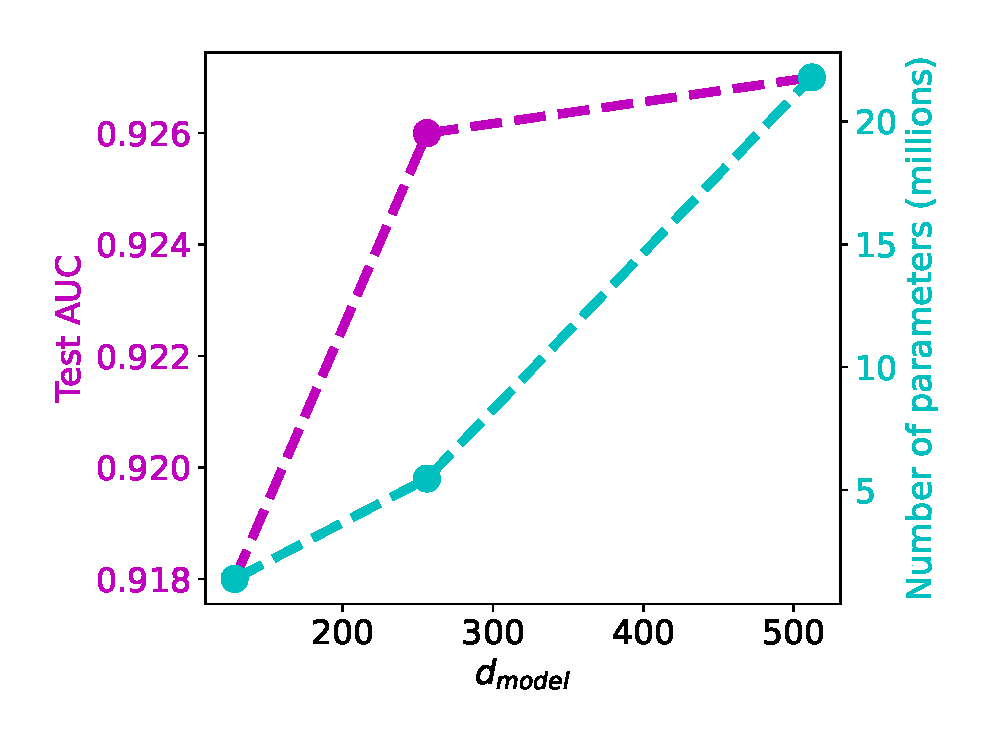
\includegraphics[width=0.8\textwidth]{dmodel_test.eps}
%\includesvg{k_mer_aggregation}
\caption{}
\label{fig:dmodel test}
\end{figure}

\subsubsection{Effects of striding}

\begin{figure}[H]
\center
\includegraphics[width=0.8\textwidth]{stride_test.eps}
%\includesvg{k_mer_aggregation}
\caption{}
\label{fig:stride}
\end{figure}

%Dataset with species labels
\subsection{Species classification}



\bibliography{data/references}{}
\bibliographystyle{unsrt}

\end{document}
